\documentclass[a4paper,12pt]{report}
\usepackage[spanish]{babel}
\usepackage[utf8]{inputenc}
\usepackage{graphicx, csquotes, longtable, array, booktabs, xparse, float, titlesec, enumitem, dingbat, soul, multicol, listings}
\usepackage[dvipsnames]{xcolor}
\usepackage[margin=2cm]{geometry}

% Añadir la bibliografía
%\usepackage[backend=biber, style=numeric, sorting=ynt]{biblatex}
%\addbibresource{memoria.bib}

% Cambia el color de los links
\usepackage{hyperref}
\hypersetup{hidelinks}

% Elimina la palabra "Capítulo" de los títulos de los capítulos
\titleformat{\chapter}[display]
  {\normalfont\bfseries}{}{0pt}{\Huge\thechapter.\space}

\titleformat{name=\chapter,numberless}[display]
  {\normalfont\bfseries}{}{0pt}{\Huge}

\titlespacing*{\chapter}{0pt}{-50pt}{20pt}

% Idioma predeterminado (Español)
\selectlanguage{spanish}

\begin{document}
  \begin{titlepage}
      \centering
      
\includegraphics[width=0.6\textwidth]{img/logo.jpg}\\
      \vspace{1cm}
      \LARGE Desarrollo Avanzado de Software\\
      \vspace{0.5cm}
      \Large Ingeniería Informática de Gestión y Sistemas de Información\\
      \vspace{3cm}
      \vspace{0.5cm}
      \Huge \textbf{UNIGO}\\
      \huge NOMBRE GRUPO\\
      \vspace{2.5cm}
      \Large Autores:\\
      \vspace{0.2cm}
      \large Dueñas Fernandez, Iñigo\\
      \large Etxaniz Monge, Eneko\\
      \large Gabiña Barañano, Xabier\\
      \large Palacios Orueta, Irune\\
      \vfill
      \today
  \end{titlepage}
  \tableofcontents
  \listoffigures
  \chapter{Introducción}
    \begin{center}
      \href{https://github.com/Xabierland/UNIGO}{Repositorio del proyecto en GitHub}
    \end{center}
    \section{Introducción del Proyecto}
      El proyecto \textbf{UNIGO - Aula Open Data de la UPV/EHU} consiste en el desarrollo de una aplicación móvil para el sistema operativo Android, orientada a facilitar el acceso al campus de Álava desde cualquier punto de la ciudad de Vitoria-Gasteiz. La aplicación integra múltiples modos de transporte (a pie, en bicicleta, en tranvía y en autobús urbano), utilizando datos abiertos provenientes de diversas fuentes oficiales, tales como el Gobierno Vasco, Euskotren y Tuvisa. Este proyecto forma parte de la asignatura de Desarrollo Avanzado de Software y ha sido desarrollado en grupo aplicando metodologías ágiles y patrones de diseño modernos, como el \textit{MVVM}, complementados con el uso de tecnologías como Firebase para la autenticación y Room para la persistencia de datos.
    \section{Propósito del Proyecto}
      El propósito principal del proyecto es diseñar y desarrollar una solución tecnológica que permita a los usuarios planificar rutas óptimas y adaptadas a sus necesidades, garantizando una movilidad eficiente y sostenible hacia el campus de Álava. Asimismo, la aplicación contempla funcionalidades adicionales, tales como el registro e inicio de sesión, la personalización de perfiles y la consulta en tiempo real de información de transporte, contribuyendo a la integración de servicios de movilidad y mejorando la experiencia de los usuarios.
    \section{Asociaciones y Ámbito de Aplicación}
      El desarrollo de la aplicación se enmarca en el aula Open Data de la UPV/EHU y cuenta con la colaboración de diversas entidades. Las principales asociaciones involucradas son:
      \begin{itemize}
        \item \textbf{Instituciones Educativas:} La UPV/EHU como impulsora del proyecto y usuario principal.
        \item \textbf{Gobierno Vasco:} Proveedor de datos abiertos esenciales para la planificación de rutas y la gestión de la movilidad urbana.
        \item \textbf{Operadores de Transporte:} Integración de información sobre servicios de transporte público (Euskotren y Tuvisa) para proporcionar rutas actualizadas y optimizadas.
      \end{itemize}
      El ámbito de aplicación abarca tanto el entorno universitario como el contexto urbano de Vitoria-Gasteiz, facilitando el acceso al campus para estudiantes, personal académico y otros usuarios.
    \section{Contexto de Negocio}
      En el contexto actual, la necesidad de optimizar la movilidad urbana y fomentar el uso de medios de transporte sostenibles es cada vez más prioritaria. La aplicación UNIGO no solo busca resolver un reto técnico mediante el uso de datos abiertos y tecnologías móviles, sino también contribuir a la reducción de la huella de carbono, promover hábitos de vida saludables y reforzar la interconexión entre servicios públicos y privados. En este sentido, el proyecto se alinea con las tendencias globales de innovación en el transporte y la digitalización de los servicios, posicionándose como una herramienta clave para el desarrollo urbano sostenible en Vitoria-Gasteiz.
    \section{Definiciones, Acrónimos y Abreviaturas}
      \begin{itemize}
        \item \textbf{UNIGO:} Nombre del proyecto orientado a resolver el reto propuesto en el aula Open Data de la UPV/EHU.
        \item \textbf{Aula Open Data:} Espacio de colaboración y aprendizaje en el que se utilizan datos abiertos para la resolución de problemas reales.
        \item \textbf{Android:} Sistema operativo móvil utilizado para el desarrollo de la aplicación.
        \item \textbf{Firebase:} Plataforma de desarrollo que ofrece servicios como autenticación, base de datos en tiempo real, entre otros.
        \item \textbf{MVVM:} Patrón de diseño (\textit{Model-View-ViewModel}) implementado en la arquitectura de la aplicación.
        \item \textbf{Room:} Biblioteca de persistencia de datos en Android que facilita la gestión de bases de datos locales.
        \item \textbf{API:} Interfaz de Programación de Aplicaciones que permite la integración y obtención de información de fuentes externas (Gobierno Vasco, Euskotren, Tuvisa).
      \end{itemize}
    \chapter{Descripción del proyecto}
      \section{Descripción del proyecto}
        La aplicación \textbf{UNIGO - Aula Open Data de la UPV/EHU} es una herramienta móvil desarrollada para el sistema operativo Android. Su objetivo es facilitar el acceso al campus de Álava desde cualquier punto de la ciudad de Vitoria-Gasteiz, integrando en una única plataforma información proporcionada por diversas fuentes oficiales. La aplicación utiliza datos abiertos de entidades como el Gobierno Vasco, Euskotren y Tuvisa, permitiendo ofrecer rutas optimizadas en función de diferentes medios de transporte:
        \begin{itemize}
          \item A pie,
          \item En bicicleta,
          \item En tranvía,
          \item En autobús urbano.
        \end{itemize}
        Entre sus funcionalidades destacan la planificación y optimización de rutas, el cálculo del tiempo estimado de llegada y, en algunos casos, estimaciones de calorías consumidas y emisiones de CO\textsubscript{2}. Además, incorpora un sistema de gestión de usuarios mediante Firebase Authentication, permitiendo el registro, personalización de perfiles y seguimiento del historial de rutas, lo cual mejora la experiencia del usuario y la calidad del servicio ofrecido.
      \section{Problema que Resuelve}
        El proyecto se orienta a superar varias problemáticas específicas del entorno urbano y académico:
        \begin{itemize}
          \item \textbf{Accesibilidad al Campus:} Facilita el acceso al campus de Álava, ofreciendo a estudiantes, profesores y personal administrativo rutas adaptadas a diferentes formas de desplazamiento.
          \item \textbf{Optimización de Desplazamientos:} Resuelve la complejidad de planificar rutas eficientes en una ciudad con múltiples opciones de transporte, proporcionando alternativas que optimizan tiempos de desplazamiento y minimizan distancias.
          \item \textbf{Integración y Actualización de Datos:} Supera el reto que supone integrar información heterogénea proveniente de diversas fuentes de datos abiertos, permitiendo al usuario disponer de información actualizada y fiable sobre los servicios de transporte.
          \item \textbf{Fomento de la Movilidad Sostenible:} Contribuye a reducir la huella de carbono y promueve hábitos de vida saludables al incentivar el uso de medios de transporte más sostenibles.
        \end{itemize}
        En definitiva, la aplicación no solo aborda los desafíos técnicos de la integración de múltiples fuentes de datos, sino que también actúa como un facilitador en la mejora de la movilidad y conectividad en el entorno urbano, beneficiando tanto a la comunidad universitaria como a la sociedad en general.
      \section{Valor del Desarrollo}
        El desarrollo de la aplicación \textbf{UNIGO} aporta un valor significativo en diferentes ámbitos:
        \begin{itemize}
          \item \textbf{Valor Tecnológico e Innovador:} La implementación de tecnologías modernas como Android Nativo, Firebase, Google Maps API y Room permite a los desarrolladores adquirir y aplicar conocimientos prácticos en un entorno real, enriqueciendo la experiencia formativa y profesional.
          \item \textbf{Impacto en la Movilidad Urbana:} Al optimizar el proceso de planificación de rutas y fomentar la utilización de medios de transporte sostenibles, el proyecto contribuye a mejorar la eficiencia en los desplazamientos hacia el campus, reduciendo tanto el tiempo de viaje como el impacto ambiental.
          \item \textbf{Beneficio Educativo:} La aplicación integra de forma práctica los contenidos teóricos vistos en clase, proporcionando un escenario de aplicación real que potencia la formación en desarrollo de software y en el manejo de datos abiertos.
          \item \textbf{Beneficios Sociales y Ambientales:} Además de mejorar la movilidad, el proyecto tiene un impacto positivo en la sociedad al promover estilos de vida saludables y sostenibles, ayudando a disminuir la congestión urbana y la contaminación atmosférica.
        \end{itemize}
        De esta manera, el desarrollo del proyecto no sólo resuelve un problema concreto de accesibilidad y movilidad urbana, sino que también se posiciona como una herramienta innovadora y formativa que contribuye al desarrollo sostenible y a la mejora de la calidad de vida de los usuarios.
  \chapter{Objetivos del proyecto}
    \section{Desarrollo del Proyecto UNIGO}
  \chapter{Arquitectura}
    \begin{figure}[H]
      \centering
      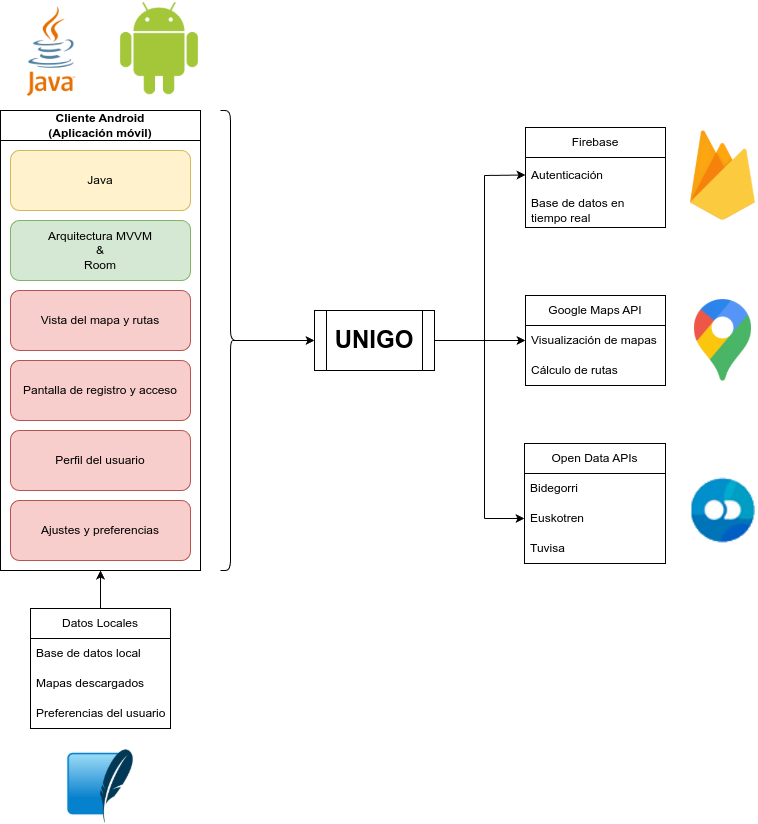
\includegraphics[width=0.8\textwidth]{img/arquitectura.png}
      \caption{Arquitectura de la aplicación UNIGO}
      \label{fig:arquitectura}
    \end{figure}
  \chapter{Herramientas}
    \section*{Git}
      Git es un sistema de control de versiones distribuido diseñado para gestionar y registrar los cambios realizados en el código fuente de un proyecto. Su capacidad para manejar ramas, fusionar desarrollos paralelos y revertir modificaciones permite una colaboración eficiente entre múltiples desarrolladores, asegurando además la trazabilidad histórica de todas las modificaciones.
    \section*{GitHub}
      GitHub es una plataforma web que integra Git para el control de versiones y facilita la colaboración en proyectos de desarrollo. Proporciona herramientas para la gestión de incidencias, solicitudes de extracción (pull requests) y revisiones de código, lo que permite un flujo de trabajo colaborativo y la integración continua. Además, GitHub facilita la difusión del proyecto mediante la publicación y documentación de código en repositorios públicos o privados.
    \section*{Markdown}
      Markdown es un lenguaje de marcado ligero que permite la elaboración de textos formateados de manera sencilla y legible tanto en su forma original como en su versión renderizada (usualmente a HTML). Su uso es común en la documentación de proyectos, facilitando la redacción de archivos README, wikis y blogs sin la complejidad de lenguajes de marcado más robustos.
    \section*{LaTeX}
      LaTeX es un sistema de composición tipográfica ampliamente utilizado para la creación de documentos científicos, técnicos y académicos de alta calidad. Permite el manejo preciso de estructuras complejas, como fórmulas matemáticas, bibliografías, tablas y gráficos, ofreciendo un control detallado sobre el formato y la presentación del documento. Su uso es particularmente habitual en entornos académicos e investigadores.
    \section*{Android Studio}
      Android Studio es el entorno de desarrollo integrado (IDE) oficial para el desarrollo de aplicaciones Android. Proporciona un conjunto completo de herramientas que incluyen editores de código, emuladores, depuradores y herramientas de análisis de rendimiento, facilitando la creación, prueba y despliegue de aplicaciones en un entorno robusto y optimizado para el sistema operativo Android.
    \section*{Visual Studio Code}
      Visual Studio Code (VS Code) es un editor de código fuente multiplataforma que ofrece soporte para numerosos lenguajes de programación y tecnologías. Su interfaz intuitiva, junto con la amplia variedad de extensiones disponibles, lo convierten en una herramienta versátil y poderosa para el desarrollo de software. La integración nativa con sistemas de control de versiones y herramientas de depuración mejora la productividad de los desarrolladores.
    \section*{Firebase}
      Firebase es una plataforma de desarrollo proporcionada por Google que integra múltiples servicios orientados al desarrollo de aplicaciones móviles y web. Entre sus características se incluyen la autenticación de usuarios, bases de datos en tiempo real, almacenamiento en la nube y análisis de datos. Estas herramientas permiten una implementación rápida y escalable de funcionalidades esenciales, facilitando el desarrollo de aplicaciones modernas y seguras.
    \section*{Google Maps API}
      Google Maps API es un conjunto de interfaces de programación que permite la integración de mapas y funcionalidades geoespaciales en aplicaciones web y móviles. Ofrece servicios de geolocalización, planificación de rutas, visualización de mapas y análisis espacial, lo cual resulta fundamental para el desarrollo de aplicaciones que requieren servicios de información geográfica en tiempo real o análisis de datos basados en la localización.
  \chapter{Alcance del proyecto}
\end{document}